\section{Associated Graded Ring}

We interject momentarily to discuss the geometric interpretation of a common construction: the associated graded ring. For a ring $R$, define the associated graded ring with respect to ideal $I$ to be
\[
    \text{gr}_I(R) = \frac{R}{I} \oplus \frac{I}{I^2} \oplus \frac{I^2}{I^3} \oplus \dots.
\]

To visualize $\text{gr}_I(R)$, we will take the following example:
\[
    R = \left( \frac{k[x,y]}{y^2 - x^2 - x^3} \right)_{(0,0)}, \quad I = \mathfrak m = (x,y) \subset R.
\]
Let $D \subset k^2$ denote the set of solutions to $y^2 - x^2 - x^3 = 0$. Then observe
\begin{itemize}
    \item $R/\mathfrak m = $ set of polynomials on $D$, identifying two polynomials if they agree at $(0,0)$. That is, $R/\mathfrak m$ represents possible values at $(0,0)$.
    \item $\mathfrak m/\mathfrak m^2 = $ set of polynomials on $D$ vanishing at $(0,0)$, identifying two polynomials if their derivatives agree. That is, $\mathfrak m/\mathfrak m^2$ represents possible first-order behavior at $(0,0)$.
    \item In general, $\mathfrak m^i/\mathfrak m^{i+1}$ represents possible $i$-th order behavior at $(0,0)$.
\end{itemize}
Thus, an element $f \in \text{gr}_{\mathfrak m}(R)$ can be interpreted as a function defined on some neighborhood of $(0,0)$ in $D$ (with finite order of vanishing at $(0,0)$) and represented as
\[
    (\text{value at (0,0)}) \oplus (\text{1st-order behavior}) \oplus (\text{2nd-order behavior}) \oplus \dots
\]
For every such $f$, observe there exists a polynomial defined on the tangent cone at $(0,0)$ with the exact same local behavior. It is easy to see this correspondance is a bijection, so we conclude that $\text{gr}_{\mathfrak m}(R) \cong$ the coordinate ring defined on the tangent cone at $(0,0)$.
\begin{figure}[H]
    \centering
    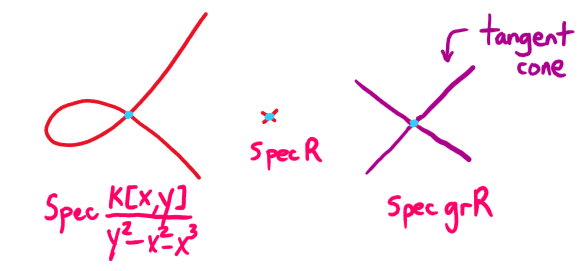
\includegraphics[width=0.6\linewidth]{figures/tangent-cone.png}
\end{figure}

[The tangent cone is a generalization of the tangent space to also handle singularities. Note if we did not localize at the singular point $(0,0)$, we would have gotten the coordinate ring over the tangent line at the point of localization.] [Also note in our example that finite order of vanishing of $f$ is key.]
%%% Local Variables:
%%% TeX-master: "main"
%%% End: